% Laporan Proyek IoT - SIC Batch 8, Selection Phase 2
% Build (from this folder): latexmk -pdf laporan.tex   (run twice without latexmk so the TOC fills in)
% Overleaf: upload the whole repository, then set latex/laporan.tex as the main document.
% Layout follows notes/format.txt; content follows "Isi Laporan .docx" in the SIC 8 guideline.

\documentclass[12pt,a4paper,oneside]{report}

% --- Language, fonts, page geometry ---------------------------------------
\usepackage[T1]{fontenc}
\usepackage[utf8]{inputenc}
\usepackage[indonesian]{babel}          % Bab, Gambar, Tabel, Daftar Isi
\usepackage{mathptmx}                   % Times New Roman look-alike
\usepackage[top=4cm,left=4cm,bottom=3cm,right=3cm]{geometry}
\usepackage{setspace}
\onehalfspacing                         % 1.5 line spacing for body text
\usepackage{indentfirst}
\setlength{\parindent}{1cm}             % first-line indent of about 1 cm

% --- Tables, figures, lists, code ------------------------------------------
\usepackage{graphicx}
\graphicspath{{../image/}{image/}}      % repo layout first, flat Overleaf upload second
\usepackage{float}
\usepackage{array,booktabs,tabularx}
\usepackage[labelfont=bf,labelsep=space,justification=centering]{caption}
\captionsetup[table]{position=above,skip=6pt}
\captionsetup[figure]{position=below,skip=6pt}
\usepackage{enumitem}
\setlist{itemsep=0pt,topsep=4pt}
\usepackage{xcolor}
\usepackage{listings}
\usepackage{etoolbox}
\usepackage[hidelinks]{hyperref}
\usepackage{url}

% Tables read better single-spaced and slightly smaller than body text;
% redefine \tablesize inside one table to shrink just that table
\newcommand{\tablesize}{\small}
\AtBeginEnvironment{tabularx}{\singlespacing\tablesize}
% Extra stretch so justified lines with long words do not run into the margin
\setlength{\emergencystretch}{3em}
\renewcommand{\arraystretch}{1.25}
\newcolumntype{L}{>{\raggedright\arraybackslash}X}
\newcolumntype{P}[1]{>{\raggedright\arraybackslash}p{#1}}

% Yellow box for parts the team still has to fill in
\newcommand{\isi}[1]{\colorbox{yellow}{\textbf{[#1]}}}

% Monospace style for topic names, pins and Serial messages in running text
\newcommand{\kode}[1]{\texttt{#1}}

% Source code listing style for the appendix
\lstset{
  basicstyle=\ttfamily\footnotesize\singlespacing,
  numbers=left, numberstyle=\tiny\color{gray}, numbersep=6pt,
  frame=single, rulecolor=\color{gray!60},
  breaklines=true, columns=fullflexible, keepspaces=true, tabsize=2,
  keywordstyle=\color{blue!60!black}\bfseries,
  commentstyle=\color{green!40!black}\itshape,
  stringstyle=\color{red!60!black},
  language=C++
}

% --- Headings: "BAB I" + title, 14 pt bold uppercase, centred ---------------
\usepackage{titlesec}
\titleformat{\chapter}[display]
  {\centering\bfseries\fontsize{14}{18}\selectfont}
  {BAB \thechapter}{0pt}{\MakeUppercase}

% Chapters are "BAB I, II, ...", but sections, figures and tables keep 1.1, 2.1, ...
\renewcommand{\thechapter}{\Roman{chapter}}
\renewcommand{\thesection}{\arabic{chapter}.\arabic{section}}
\renewcommand{\thefigure}{\arabic{chapter}.\arabic{figure}}
\renewcommand{\thetable}{\arabic{chapter}.\arabic{table}}

% Table of contents / lists in Indonesian report style: "BAB I", "Gambar 2.1", "Tabel 2.1"
\usepackage[titles]{tocloft}
\renewcommand{\cftchappresnum}{BAB~}
\setlength{\cftchapnumwidth}{4.2em}
\renewcommand{\cftfigpresnum}{Gambar~}
\setlength{\cftfignumwidth}{5.5em}
\renewcommand{\cfttabpresnum}{Tabel~}
\setlength{\cfttabnumwidth}{5em}
\titlespacing*{\chapter}{0pt}{0pt}{24pt}
\titleformat{\section}{\bfseries\normalsize}{\thesection}{0.75em}{}
\titleformat{\subsection}{\bfseries\normalsize}{\thesubsection}{0.75em}{}
% Unnumbered front-matter headings use the same look
\titleformat{name=\chapter,numberless}[block]
  {\centering\bfseries\fontsize{14}{18}\selectfont}{}{0pt}{\MakeUppercase}

\begin{document}

% =========================================================================
% COVER
% =========================================================================
\begin{titlepage}
  \centering
  \singlespacing
  {\fontsize{16}{20}\selectfont\bfseries LAPORAN PROYEK INTERNET OF THINGS\par}
  \vspace{1.2cm}
  {\large\bfseries Sistem Deteksi Kebocoran Gas LPG dengan Penutup Otomatis Tuas Regulator Berbasis ESP32 dan Pemantauan MQTT\par}
  \vspace{1cm}
  Disusun untuk Study Case Selection Phase 2:\\
  IoT Device and Hardware Discovery\\
  Samsung Innovation Campus Batch 8\par
  \vspace{1.5cm}
  
\includegraphics[width=4.5cm]{logo-its.png}
  \vfill
  {\bfseries Disusun oleh:\par}
  \vspace{0.3cm}
  Nama tim: Malas Mikir Nama\par
  \vspace{0.3cm}
  \begin{tabular}{l l}
    Frenaldy Bestabba Hasugian & (5025241156) \\
    Muhammad Sayyid Tsabit     & (5024241013) \\
    Nicholas                   & (5022241065) \\
    Mitra Partogi              & (5025241017) \\
  \end{tabular}\par
  \vfill
  {\bfseries Institut Teknologi Sepuluh Nopember\par}
  2026\par
\end{titlepage}

% =========================================================================
% FRONT MATTER (roman page numbers)
% =========================================================================
\pagenumbering{roman}
\setcounter{page}{2}

\chapter*{Kata Pengantar}
\addcontentsline{toc}{chapter}{KATA PENGANTAR}
Puji syukur kami panjatkan kepada Tuhan Yang Maha Esa karena laporan proyek Internet of Things berjudul \emph{Sistem Deteksi Kebocoran Gas LPG dengan Penutup Otomatis Tuas Regulator Berbasis ESP32 dan Pemantauan MQTT} dapat diselesaikan. Laporan ini disusun untuk memenuhi Study Case Selection Phase 2: IoT Device and Hardware Discovery pada program Samsung Innovation Campus Batch 8.

Laporan ini menjelaskan proses ideasi, pemilihan perangkat, perancangan rangkaian, pemrograman ESP32, komunikasi MQTT, visualisasi data, hingga pengujian sistem pada simulator Wokwi. Kami menyadari laporan ini masih memiliki kekurangan, sehingga kritik dan saran yang membangun sangat kami harapkan.

\vspace{1cm}
\begin{flushright}
Surabaya, 30 Oktober 2026\\[1.5cm]
Tim Malas Mikir Nama
\end{flushright}

% Each entry is recorded at the top of its own page, so the TOC shows its first page
\cleardoublepage\addcontentsline{toc}{chapter}{DAFTAR ISI}
\tableofcontents
\cleardoublepage\addcontentsline{toc}{chapter}{DAFTAR GAMBAR}
\listoffigures
\cleardoublepage\addcontentsline{toc}{chapter}{DAFTAR TABEL}
\listoftables

% =========================================================================
% BAB I
% =========================================================================
\cleardoublepage
\pagenumbering{arabic}

\chapter{PENDAHULUAN}

\section{Latar Belakang}
Liquefied Petroleum Gas (LPG) atau gas elpiji adalah bahan bakar memasak yang dipakai luas di rumah tangga dan usaha kuliner di Indonesia, terutama sejak program konversi minyak tanah ke LPG yang dimulai pemerintah pada 2007. Kebocoran pada tabung, regulator, atau selang dapat memicu kebakaran dan ledakan jika gas yang bocor bertemu sumber api.

LPG lebih berat daripada udara, sehingga gas yang bocor cenderung mengumpul di dekat lantai dan tidak cepat hilang. Produsen menambahkan zat pembau agar kebocoran tercium, tetapi cara ini bergantung pada penghuni yang sedang berada di lokasi, terjaga, dan menyadari baunya. Saat penghuni tidur, berada di ruangan lain, atau tidak di rumah, kebocoran dapat berlangsung tanpa diketahui. Selain itu, regulator LPG rumah tangga yang umum dipakai hanya memiliki tuas manual, sehingga aliran gas baru tertutup jika ada orang yang memutarnya.

Dari sisi Keselamatan dan Kesehatan Kerja (K3), tindakan yang benar saat terjadi kebocoran adalah menutup aliran gas dari sumbernya dengan memutar tuas regulator ke posisi OFF. Mencabut selang dari regulator saat tuas masih ON justru berbahaya, karena gas dari tabung akan keluar bebas ke ruangan. Tindakan ini juga harus dilakukan tanpa menimbulkan percikan api, misalnya tanpa menyalakan kompor atau sakelar listrik.

Proyek ini merancang sistem berbasis Internet of Things (IoT) yang menjalankan langkah K3 tersebut secara otomatis: mendeteksi kebocoran gas, memutar tuas regulator ke posisi OFF menggunakan motor stepper, memberi peringatan suara kepada orang di sekitar lokasi, dan mengirim status ke dashboard agar kondisi dapat dipantau dari jarak jauh. Penggerak tuas dirancang untuk dipasang di luar regulator (non-invasif), sehingga bagian kedap gas regulator tidak perlu dibongkar. Seluruh rangkaian dirancang dan diuji pada simulator Wokwi menggunakan mikrokontroler ESP32.

\section{Problem Statement}
\begin{enumerate}
  \item Bagaimana mendeteksi kebocoran gas LPG secara otomatis tanpa bergantung pada indra penciuman penghuni?
  \item Bagaimana sistem menutup aliran gas dari sumbernya secara otomatis dengan cara yang aman menurut prinsip K3, sekaligus memperingatkan orang di sekitar lokasi?
  \item Bagaimana memastikan alarm tidak mati dengan sendirinya sebelum kondisi diperiksa oleh manusia?
  \item Bagaimana status sistem dapat dipantau dari jarak jauh?
\end{enumerate}

\section{Tujuan}
\begin{enumerate}
  \item Membaca sensor gas MQ-2 dengan ESP32 untuk mendeteksi kebocoran gas.
  \item Menggerakkan motor stepper untuk memutar tuas regulator LPG dari posisi ON ke OFF saat kebocoran terdeteksi, dan membunyikan buzzer ketika sensor PIR mendeteksi keberadaan orang.
  \item Menerapkan alarm terkunci (\emph{latching}) yang hanya dapat dimatikan dengan tombol reset.
  \item Mengirim data sensor dan status alarm melalui MQTT ke broker publik EMQX, lalu menampilkannya pada dashboard Python.
\end{enumerate}

\section{Target User dan Use Case}
Target pengguna sistem ini adalah:
\begin{itemize}
  \item Rumah tangga yang memakai kompor LPG, terutama yang dapurnya sering ditinggal atau dihuni lansia yang kepekaan penciumannya sudah menurun.
  \item Usaha kuliner kecil seperti warung makan yang memakai beberapa tabung LPG setiap hari.
  \item Pengelola kos atau asrama dengan dapur bersama yang tidak selalu diawasi.
\end{itemize}

Skenario penggunaan: saat terjadi kebocoran di dapur, sensor gas mendeteksinya dan sistem langsung mengunci alarm. Motor stepper memutar tuas regulator ke posisi OFF sehingga aliran gas dari tabung terhenti. Jika ada orang yang masuk ke area dapur, sensor PIR mendeteksinya dan buzzer berbunyi sebagai peringatan agar orang tersebut tidak menyalakan api atau sakelar listrik. Pada saat yang sama, status kebocoran terkirim ke dashboard sehingga pemilik dapat memantaunya dari tempat lain. Setelah lokasi diperiksa dan dinyatakan aman, pengguna menekan tombol reset; motor memutar tuas kembali ke posisi ON dan sistem kembali siaga.

% =========================================================================
% BAB II
% =========================================================================
\chapter{PERANCANGAN SISTEM}

\section{Arsitektur Sistem}
Sistem mengikuti alur IoT: \emph{sensing}, \emph{processing}, \emph{actuation}, \emph{communication}, dan \emph{visualization}. Peran setiap lapisan dirangkum pada Tabel~\ref{tab:arsitektur}.

\begin{table}[H]
  \caption{Arsitektur sistem per lapisan IoT}
  \label{tab:arsitektur}
  \begin{tabularx}{\textwidth}{P{3.2cm} L L}
    \toprule
    \textbf{Lapisan} & \textbf{Komponen} & \textbf{Peran} \\
    \midrule
    Input / Sensing & Sensor gas MQ-2, sensor PIR, push button & Mendeteksi gas, keberadaan orang, dan perintah reset \\
    Processing / Logic & ESP32 DevKit V1 & Menjalankan logika alarm terkunci dan mengendalikan aktuator \\
    Output / Actuation & Driver A4988 dan motor stepper NEMA 17, buzzer & Menggerakkan aktuator dan memberi peringatan suara \\
    Communication & Serial Monitor, WiFi, MQTT (broker publik EMQX) & Mengirim log debugging dan data status \\
    Visualization & Google Colab (paho-mqtt dan Matplotlib) dan dashboard web & Menampilkan status sensor dan aktuator secara live \\
    \bottomrule
  \end{tabularx}
\end{table}

Data mengalir dari sensor gas, sensor PIR, dan tombol ke ESP32. ESP32 memutuskan respons dan mengendalikan motor stepper serta buzzer. Secara bersamaan, ESP32 mengirim log ke Serial Monitor dan data status melalui MQTT ke broker publik EMQX (\kode{broker.emqx.io}), lalu dashboard Python di Google Colab dan dashboard web membaca data tersebut dari broker. Alur ini digambarkan pada Gambar~\ref{fig:blok}.

\begin{figure}[H]
  \centering
  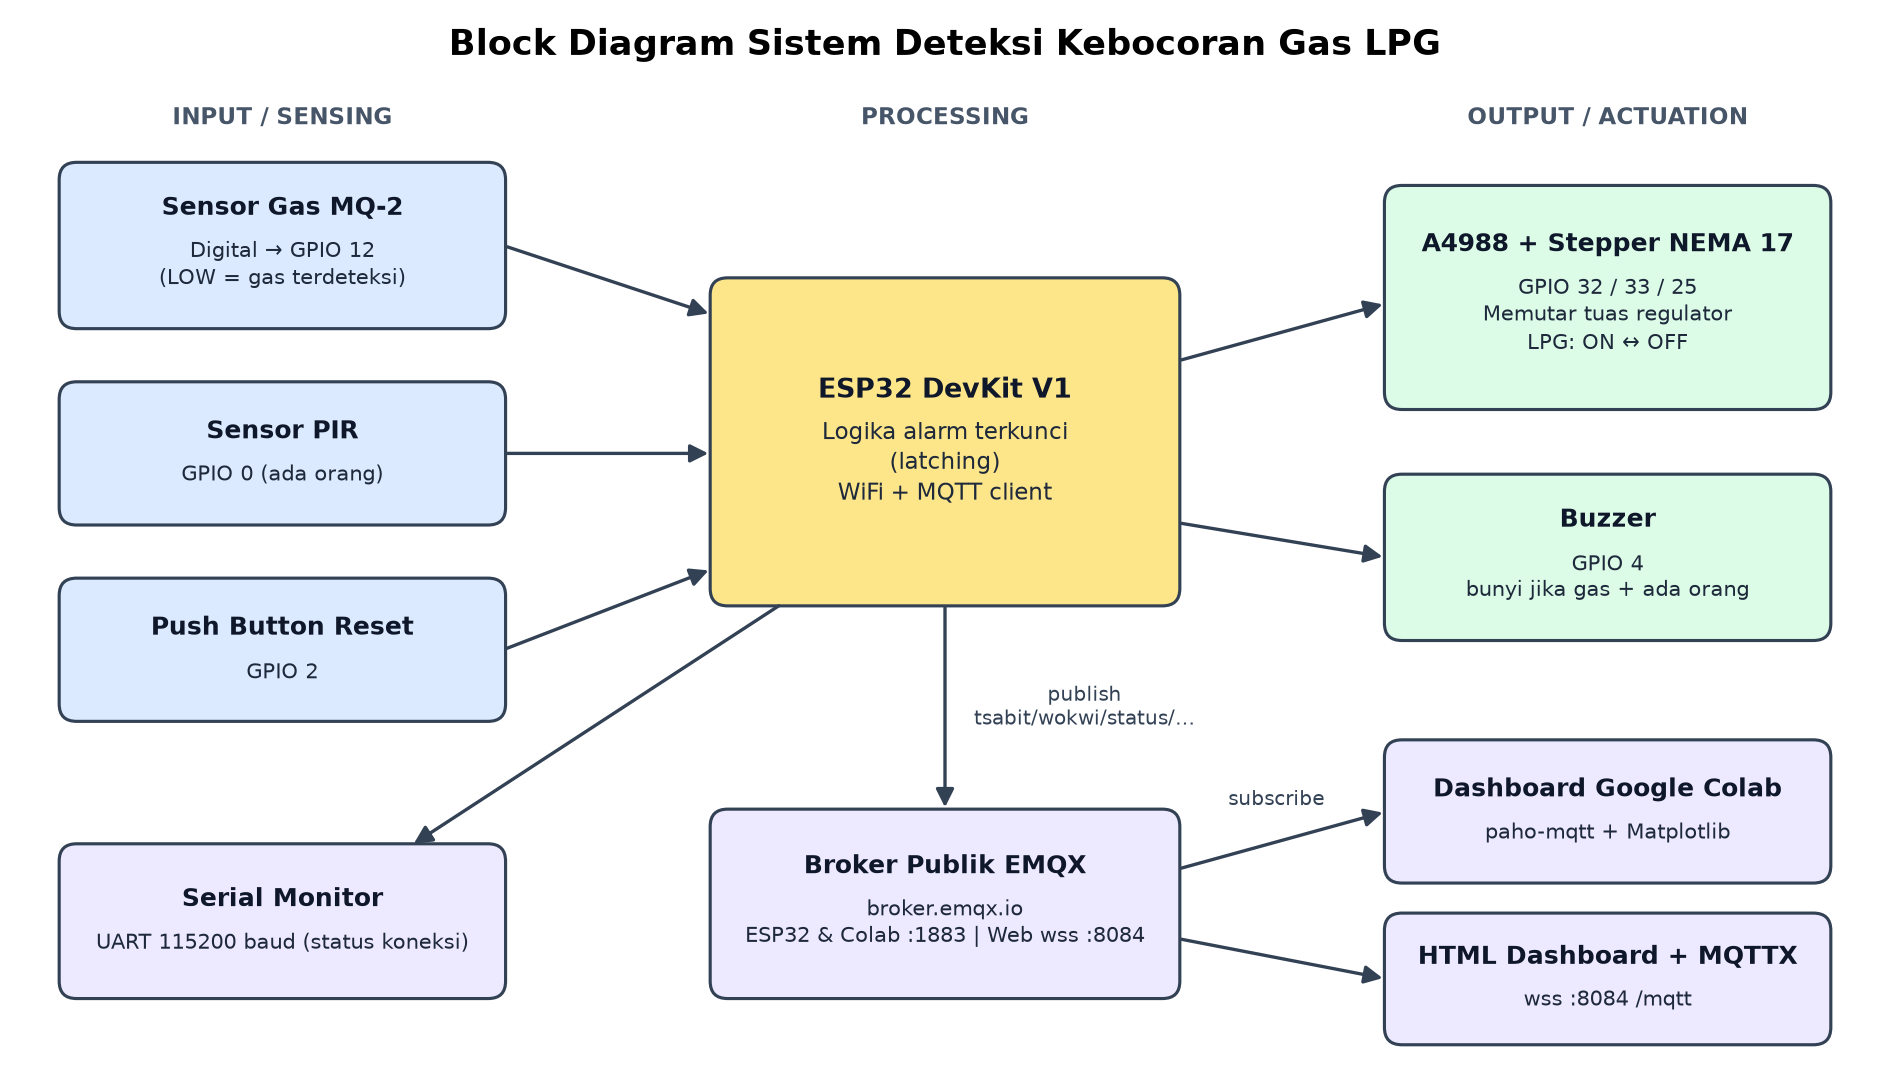
\includegraphics[width=\textwidth]{block-diagram.png}
  \caption{Block diagram sistem deteksi kebocoran gas LPG}
  \label{fig:blok}
\end{figure}

\section{Daftar Komponen dan Alasan Pemilihan}
Komponen dipilih berdasarkan kebutuhan use case dan ketersediaannya di Wokwi, seperti terlihat pada Tabel~\ref{tab:komponen}.

\begin{table}[H]
  \caption{Daftar komponen dan alasan pemilihan}
  \label{tab:komponen}
  \begin{tabularx}{\textwidth}{P{3cm} P{3.2cm} L}
    \toprule
    \textbf{Komponen} & \textbf{Fungsi} & \textbf{Alasan Pemilihan} \\
    \midrule
    ESP32 DevKit V1 & Controller utama & Ditetapkan oleh brief; memiliki WiFi bawaan untuk MQTT \\
    Sensor gas MQ-2 & Mendeteksi kebocoran gas & Peka terhadap gas mudah terbakar termasuk LPG; output digitalnya langsung menunjukkan ada atau tidaknya gas berdasarkan ambang yang diatur di modul \\
    Sensor PIR & Mendeteksi keberadaan orang & Mendeteksi panas tubuh yang bergerak, sehingga peringatan hanya dibunyikan ketika ada orang di lokasi \\
    Motor stepper NEMA 17 & Pemutar tuas regulator ON/OFF & Posisinya dapat dihitung per langkah, sehingga motor kembali tepat ke posisi awal tanpa sensor posisi \\
    Driver A4988 & Penggerak motor stepper & Pin ESP32 tidak mampu mengalirkan arus koil motor; A4988 cukup dikendalikan dengan sinyal STEP dan DIR \\
    Buzzer & Peringatan suara & Indikator sederhana untuk memperingatkan orang di sekitar lokasi \\
    Push button & Reset alarm & Memastikan alarm hanya dimatikan oleh manusia setelah kondisi diperiksa \\
    \bottomrule
  \end{tabularx}
\end{table}

\section{Rangkaian dan Wiring}
Rangkaian dibuat di Wokwi (Gambar~\ref{fig:rangkaian}). Sensor gas dan sensor PIR mendapat daya 3V3 dari ESP32. Seluruh ground terhubung ke GND ESP32 agar semua sinyal diukur terhadap titik nol yang sama. Hal penting pada wiring:
\begin{itemize}
  \item Pin ENABLE A4988 dikendalikan GPIO 25 dan bersifat aktif-LOW: LOW menghidupkan driver, HIGH mematikannya agar motor tidak panas saat diam.
  \item Driver A4988 hanya dikabel pada pin kendali (STEP, DIR, ENABLE) dan keempat output koil. Catu daya motor (VMOT) tidak diperlukan pada simulasi Wokwi, tetapi wajib pada perangkat keras nyata.
  \item Koil motor terhubung ke pasangan output 1A/1B untuk koil A dan 2A/2B untuk koil B.
  \item Tombol reset menghubungkan GPIO 2 ke GND, dan program mengaktifkan resistor pull-down internal pada pin tersebut. Program menganggap tombol ditekan ketika pin terbaca HIGH.
  \item Sensor gas memakai output digital yang terhubung ke GPIO 12. Modul bersifat aktif-LOW, sehingga LOW berarti gas terdeteksi.
\end{itemize}

\begin{figure}[H]
  \centering
  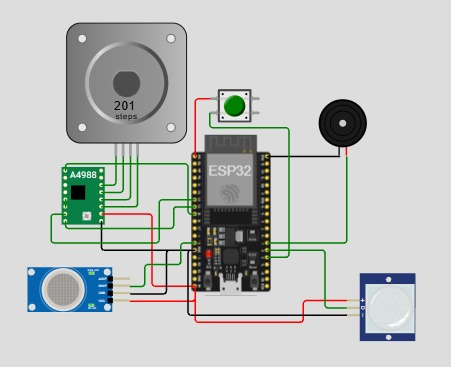
\includegraphics[width=0.8\textwidth]{rangkaian.jpeg}
  \caption{Rangkaian sistem pada simulator Wokwi}
  \label{fig:rangkaian}
\end{figure}

Link project Wokwi tercantum pada Lampiran.

\section{Pin dan GPIO}
Penggunaan pin ESP32 dirangkum pada Tabel~\ref{tab:pin}.

\begin{table}[H]
  \caption{Penggunaan pin ESP32}
  \label{tab:pin}
  \begin{tabularx}{\textwidth}{P{1.7cm} P{3.2cm} P{3.7cm} L}
    \toprule
    \textbf{Pin ESP32} & \textbf{Terhubung ke} & \textbf{Mode} & \textbf{Fungsi} \\
    \midrule
    GPIO 32 & A4988 STEP & OUTPUT & Pulsa langkah motor \\
    GPIO 33 & A4988 DIR & OUTPUT & Arah putaran motor \\
    GPIO 25 & A4988 ENABLE & OUTPUT & Menghidupkan atau mematikan driver (aktif-LOW) \\
    GPIO 12 & MQ-2 (output digital) & INPUT & Deteksi gas (LOW berarti gas terdeteksi) \\
    GPIO 0 & PIR OUT & INPUT & Deteksi keberadaan orang \\
    GPIO 2 & Push button & INPUT\_PULLDOWN & Reset alarm \\
    GPIO 4 & Buzzer & OUTPUT & Peringatan suara \\
    TX / RX & Serial Monitor & UART 115200 baud & Status koneksi WiFi dan MQTT \\
    \bottomrule
  \end{tabularx}
\end{table}

% =========================================================================
% BAB III
% =========================================================================
\chapter{IMPLEMENTASI PROGRAM}

\section{Logika Program}
Program ditulis dalam bahasa C++ (Arduino) untuk ESP32 dengan alur kerja sebagai berikut:
\begin{enumerate}
  \item Saat menyala, ESP32 mengatur mode setiap pin, mematikan driver motor dan buzzer, lalu menunggu sampai WiFi tersambung dan mengatur alamat broker MQTT.
  \item Pada setiap putaran loop, ESP32 memastikan koneksi MQTT aktif, membaca sensor gas, sensor PIR, dan tombol reset, lalu mengirim status yang berubah ke broker. Modul MQ-2 bersifat aktif-LOW, sehingga nilai LOW berarti gas terdeteksi.
  \item Jika gas terdeteksi, program masuk ke blok alarm. Blok ini hanya dapat ditinggalkan dengan menekan tombol reset, sehingga alarm tetap aktif walaupun kadar gas sudah turun.
  \item Di dalam blok alarm, motor stepper bergerak 200 langkah (satu putaran pada mode full-step) satu kali untuk memutar tuas regulator ke posisi OFF, dan posisinya dicatat dalam variabel \kode{count}. Pada simulasi, satu putaran ini merepresentasikan gerakan tuas dari ON ke OFF; rasio gir dan sudut tuas sebenarnya ditentukan saat prototipe fisik dibuat.
  \item Selama alarm aktif, program membaca sensor PIR. Buzzer berbunyi ketika ada orang dan mati ketika tidak ada orang.
  \item Saat tombol reset ditekan, buzzer dimatikan dan motor bergerak mundur 200 langkah, sehingga tuas kembali ke posisi ON. Setelah itu sistem kembali siaga.
\end{enumerate}

Alarm dibuat terkunci karena kadar gas dapat turun sesaat, misalnya karena tertiup angin, padahal sumber kebocoran belum ditangani. Dengan alarm terkunci, sistem baru kembali normal setelah manusia memeriksa lokasi dan menekan tombol reset. Kode program lengkap tercantum pada Lampiran.

\section{Komunikasi Serial}
Serial Monitor (115200 baud) dipakai untuk debugging. Serial Monitor menampilkan proses koneksi ke WiFi dan broker MQTT, sedangkan perubahan status sensor dan aktuator dipantau melalui MQTT. Daftar pesan tercantum pada Tabel~\ref{tab:serial}.

\begin{table}[H]
  \caption{Pesan Serial Monitor}
  \label{tab:serial}
  \begin{tabularx}{\textwidth}{P{7.5cm} L}
    \toprule
    \textbf{Pesan} & \textbf{Kondisi} \\
    \midrule
    \kode{[WiFi] Connecting to Wokwi-GUEST...} & ESP32 mulai menyambung ke WiFi \\
    \kode{[WiFi] Connected!} & WiFi tersambung \\
    \kode{[MQTT] Connecting to broker.emqx.io... CONNECTED!} & Koneksi ke broker publik EMQX berhasil \\
    \bottomrule
  \end{tabularx}
\end{table}

\section{Komunikasi MQTT}
ESP32 terhubung ke WiFi, lalu ke broker publik EMQX (\kode{broker.emqx.io}) melalui MQTT pada port 1883. Dashboard Colab memakai port yang sama, sedangkan dashboard web di browser memakai MQTT over WebSocket aman (wss) pada port 8084 dengan path \kode{/mqtt}, karena browser tidak dapat membuka koneksi TCP langsung seperti ESP32. Broker ini dipakai karena paket gratis HiveMQ Cloud sudah tidak tersedia untuk pengguna baru; broker publik EMQX gratis, tidak memerlukan akun, dan tetap memakai protokol MQTT standar, sehingga penguji dapat menjalankan simulasi dan dashboard tanpa kredensial.

Setiap komponen memiliki topic sendiri di bawah awalan \path|tsabit/wokwi/status/| dengan payload berupa teks. Status dikirim dengan dua cara: segera ketika nilainya berubah, dan secara rutin setiap 1 detik agar dashboard yang baru terhubung langsung mendapat kondisi terkini. Pesan dikirim dengan QoS 0 tanpa retain. Topic dan payload yang dipakai tercantum pada Tabel~\ref{tab:topic}.

\begin{table}[H]
  \caption{Topic dan payload MQTT}
  \label{tab:topic}
  \begin{tabularx}{\textwidth}{P{5.4cm} P{3.7cm} L}
    \toprule
    \textbf{Topic} & \textbf{Payload} & \textbf{Arti} \\
    \midrule
    \kode{tsabit/wokwi/status/asap} & \kode{ADA\_ASAP} atau \kode{AMAN} & Gas terdeteksi atau udara normal \\
    \kode{tsabit/wokwi/status/pir} & \kode{GERAKAN\_DETECTED} atau \kode{NORMAL} & Ada gerakan orang atau area kosong \\
    \kode{tsabit/wokwi/status/buzzer} & \kode{BUNYI} atau \kode{DIAM} & Status buzzer peringatan \\
    \kode{tsabit/wokwi/status/motor} & \kode{BERPUTAR} atau \kode{DIAM} & Status motor penggerak tuas regulator \\
    \kode{tsabit/wokwi/status/button} & \kode{PRESSED} atau \kode{RELEASED} & Status tombol reset \\
    \bottomrule
  \end{tabularx}
\end{table}

Nama topic \kode{asap} dan payload \kode{ADA\_ASAP} mengikuti penamaan di program; yang dideteksi sistem adalah kebocoran gas LPG. Karena payload berupa teks biasa, pesan dapat dibaca langsung di aplikasi MQTTX tanpa perlu diolah.

\section{Dashboard dan Visualisasi}
Dashboard utama dibuat di Google Colab menggunakan pustaka paho-mqtt untuk menerima data dan Matplotlib untuk visualisasi. Notebook berlangganan ke topic \path|tsabit/wokwi/#| dan memperbarui tampilan setiap 1 detik, dengan isi sebagai berikut:
\begin{itemize}
  \item Lima grafik status yang masing-masing bernilai 0 atau 1: sensor gas, sensor PIR, buzzer, motor stepper, dan tombol reset.
  \item Sumbu waktu dalam detik yang menampilkan 20 titik data terakhir, sehingga urutan perubahan status terlihat jelas.
  \item Sebagai pelengkap, dashboard web berbasis HTML dan JavaScript menampilkan kelima status sebagai kartu berwarna yang berubah secara real-time melalui WebSocket.
  \item Pesan juga dapat dipantau langsung dengan aplikasi MQTTX dengan berlangganan ke topic yang sama.
\end{itemize}

\begin{figure}[H]
  \centering
  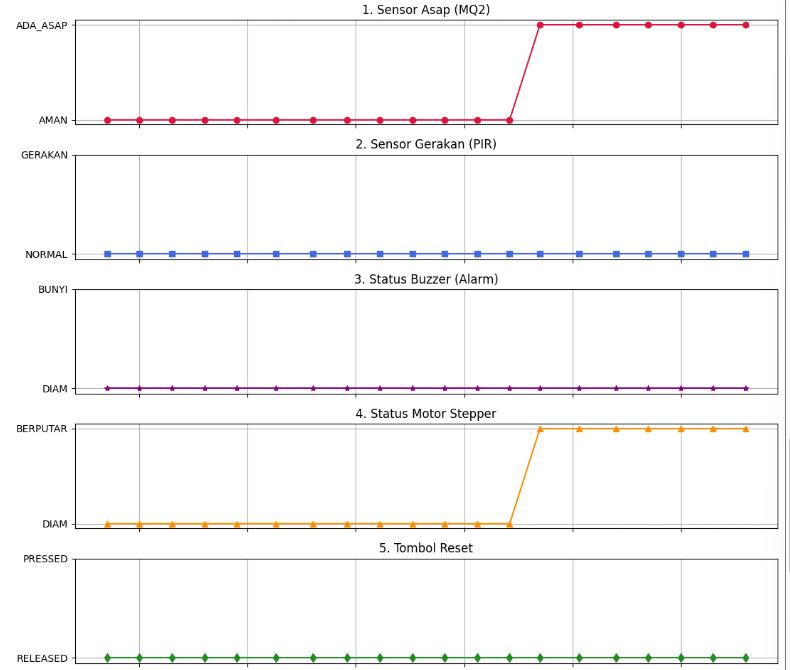
\includegraphics[width=0.85\textwidth]{dashboard.png}
  \caption{Dashboard Google Colab saat kebocoran gas terdeteksi}
  \label{fig:dashboard}
\end{figure}

% =========================================================================
% BAB IV
% =========================================================================
\chapter{PENGUJIAN}

\section{Skenario Pengujian}
Pengujian dilakukan pada simulator Wokwi dengan dashboard Colab berjalan bersamaan. Pengujian mencakup kondisi normal (TC1) dan kondisi abnormal (TC2 sampai TC4). Skenario dan hasilnya tercatat pada Tabel~\ref{tab:uji}, dengan bukti berupa screenshot pada subbab berikutnya.

\begin{table}[H]
  \caption{Skenario dan hasil pengujian}
  \label{tab:uji}
  \renewcommand{\tablesize}{\footnotesize}  % six columns: shrink this table only
  \begin{tabularx}{\textwidth}{P{0.9cm} P{1.7cm} P{2cm} L L P{1.5cm}}
    \toprule
    \textbf{ID} & \textbf{Skenario} & \textbf{Input / Kondisi} & \textbf{Hasil yang Diharapkan} & \textbf{Hasil Aktual} & \textbf{Status} \\
    \midrule
    TC1 & Kondisi normal & Gas rendah, tidak ada gerakan & Buzzer dan motor diam; dashboard menampilkan AMAN, NORMAL, DIAM, DIAM, dan RELEASED & Dengan kadar gas 10 ppm, motor dan buzzer diam; kelima grafik dashboard tetap pada AMAN, NORMAL, DIAM, DIAM, dan RELEASED (Gambar~\ref{fig:tc1}) & Berhasil \\
    TC2 & Gas terdeteksi tanpa orang & Kadar gas dinaikkan di Wokwi, PIR diam & Alarm terkunci, motor bergerak 200 langkah, buzzer diam; dashboard menampilkan ADA\_ASAP dan motor BERPUTAR & Saat kadar gas dinaikkan ke 457 ppm, dashboard berubah ke ADA\_ASAP dan motor BERPUTAR, sedangkan buzzer tetap DIAM karena PIR NORMAL (Gambar~\ref{fig:tc2}) & Berhasil \\
    TC3 & Gas terdeteksi dan ada orang & Saat alarm aktif, PIR dipicu & Buzzer berbunyi; dashboard menampilkan GERAKAN\_\allowbreak DETECTED dan BUNYI & Setelah gerakan disimulasikan, dashboard menampilkan GERAKAN dan buzzer BUNYI; penghitung langkah stepper di Wokwi menunjukkan 201 (Gambar~\ref{fig:tc3}) & Berhasil \\
    TC4 & Reset & Tombol reset ditekan saat alarm aktif & Buzzer mati, motor mundur 200 langkah; dashboard menampilkan PRESSED, lalu motor DIAM & Setelah gas diturunkan dan tombol ditekan, dashboard menampilkan PRESSED sesaat, lalu motor DIAM; penghitung langkah turun dari 201 ke 1, artinya motor mundur 200 langkah (Gambar~\ref{fig:tc4}) & Berhasil \\
    \bottomrule
  \end{tabularx}
\end{table}

\section{Screenshot dan Output}
Setiap screenshot memperlihatkan dashboard Google Colab (kiri) serta rangkaian dan Serial Monitor Wokwi (kanan) pada saat yang sama. Serial Monitor pada semua gambar menunjukkan ESP32 berhasil terhubung ke WiFi dan broker MQTT.

\begin{figure}[H]
  \centering
  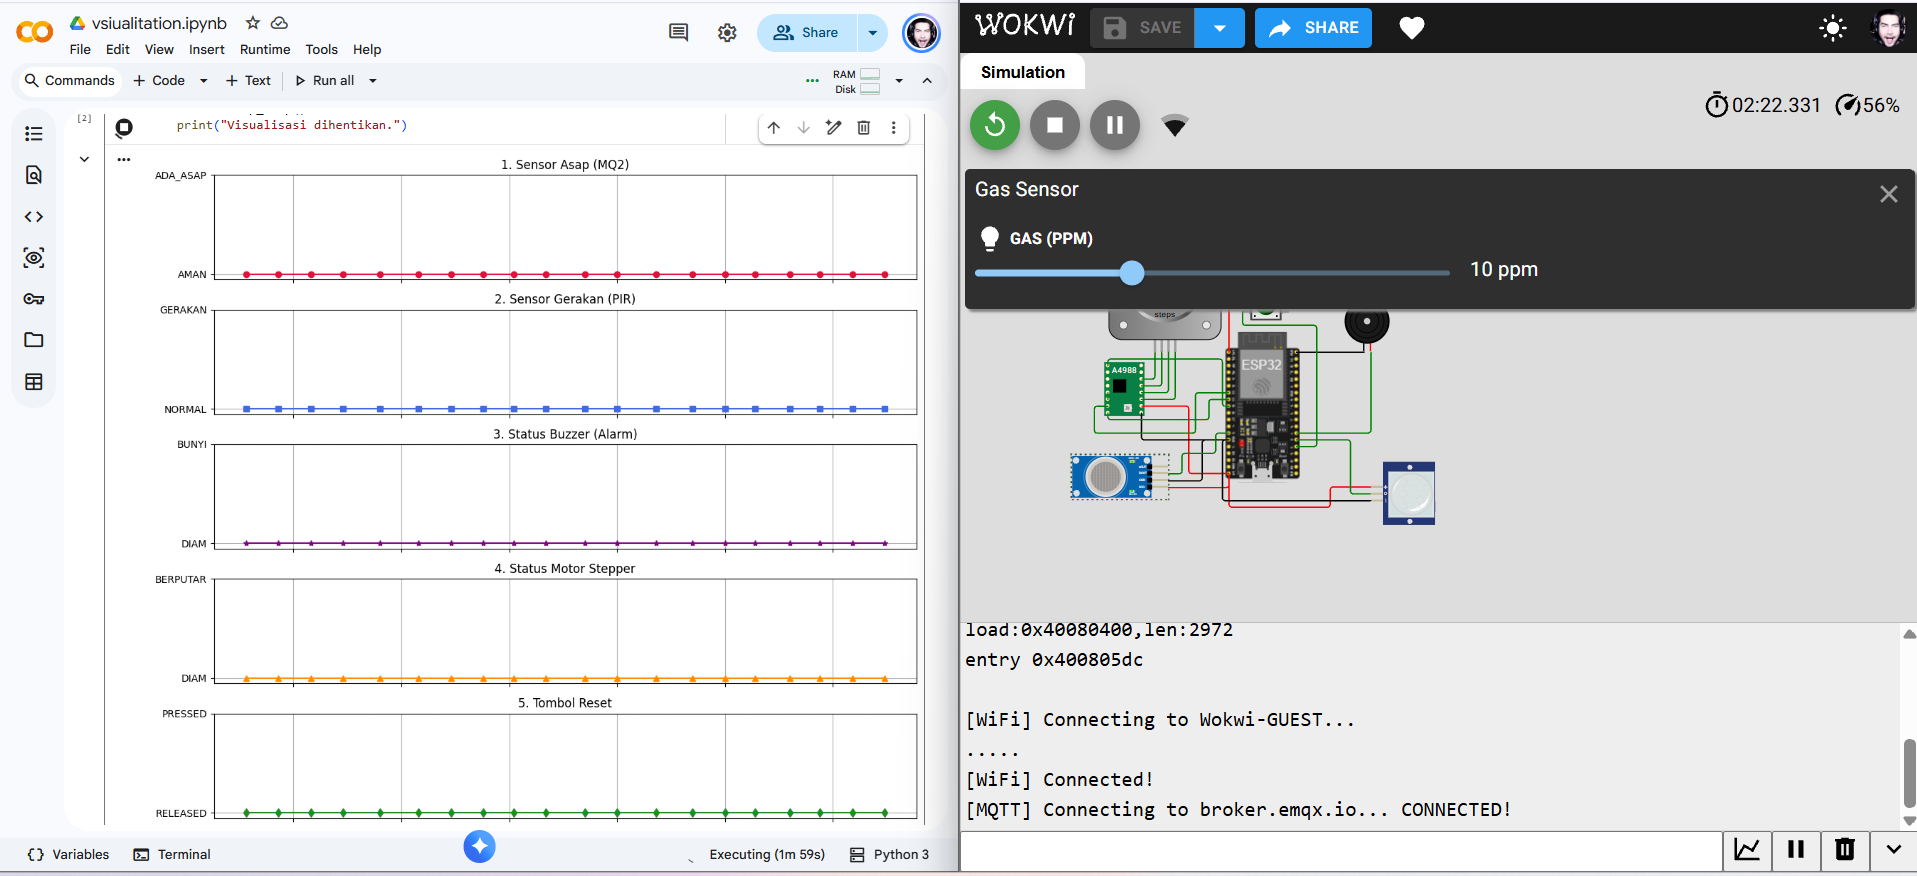
\includegraphics[width=\textwidth]{tc1.png}
  \caption{TC1: kondisi normal dengan kadar gas 10 ppm}
  \label{fig:tc1}
\end{figure}

\begin{figure}[H]
  \centering
  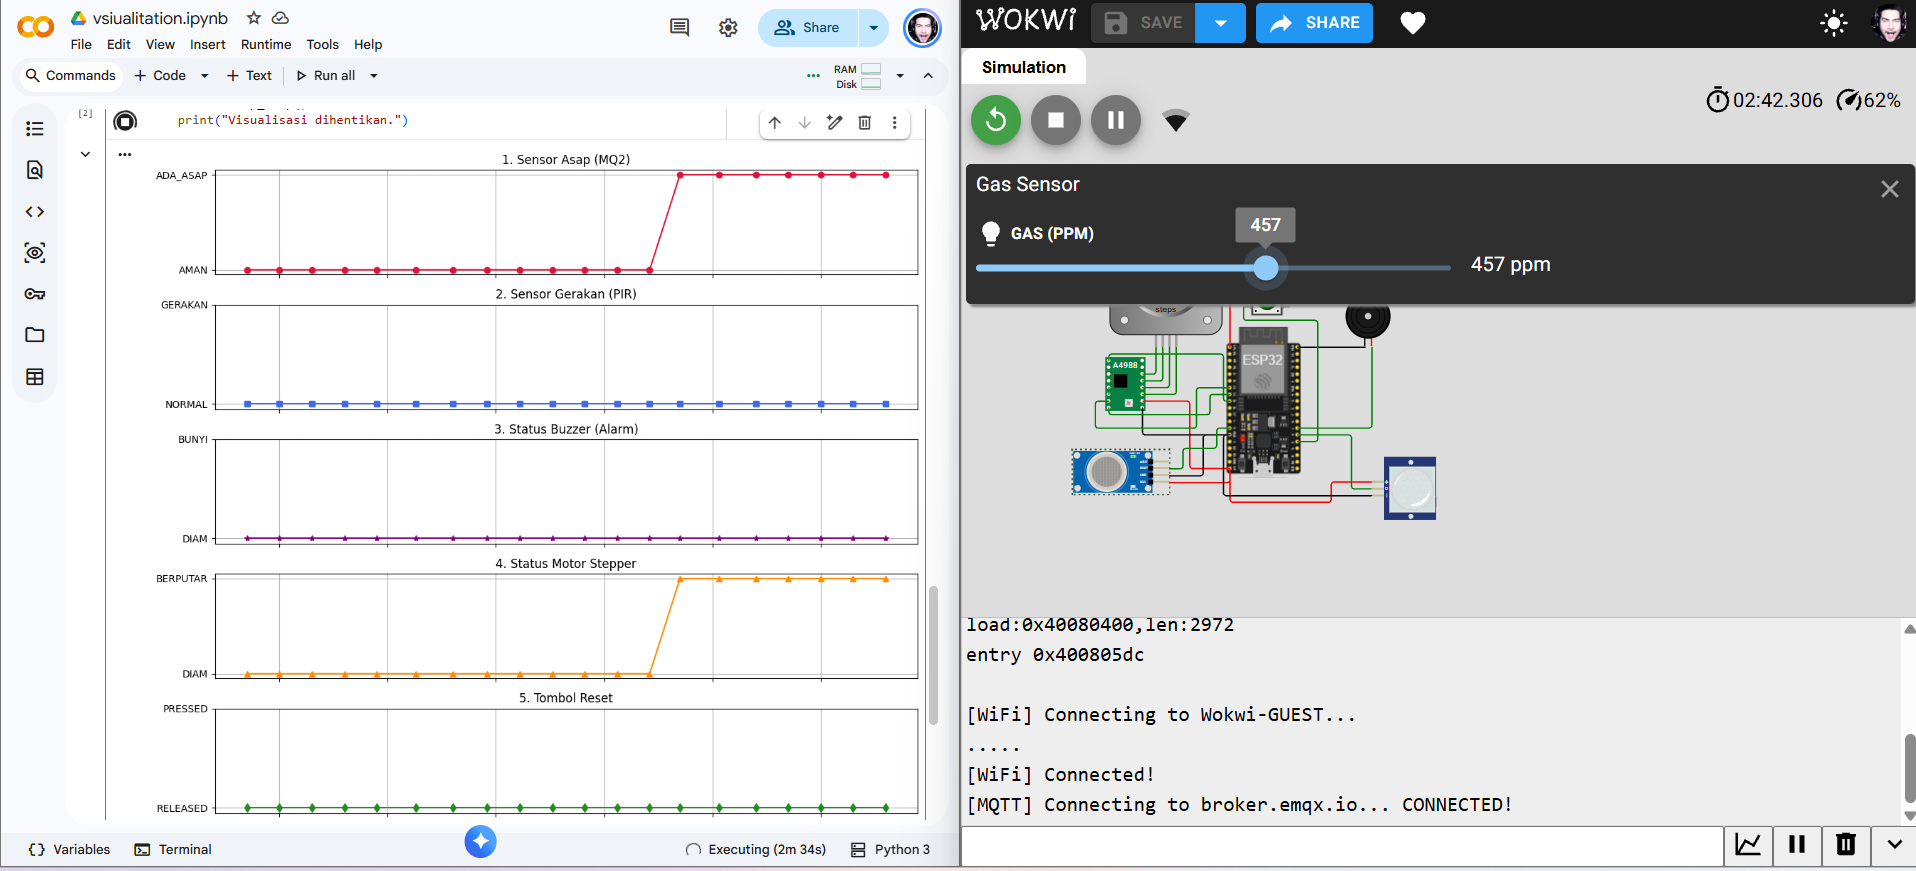
\includegraphics[width=\textwidth]{tc2.png}
  \caption{TC2: gas terdeteksi (457 ppm) tanpa orang}
  \label{fig:tc2}
\end{figure}

\begin{figure}[H]
  \centering
  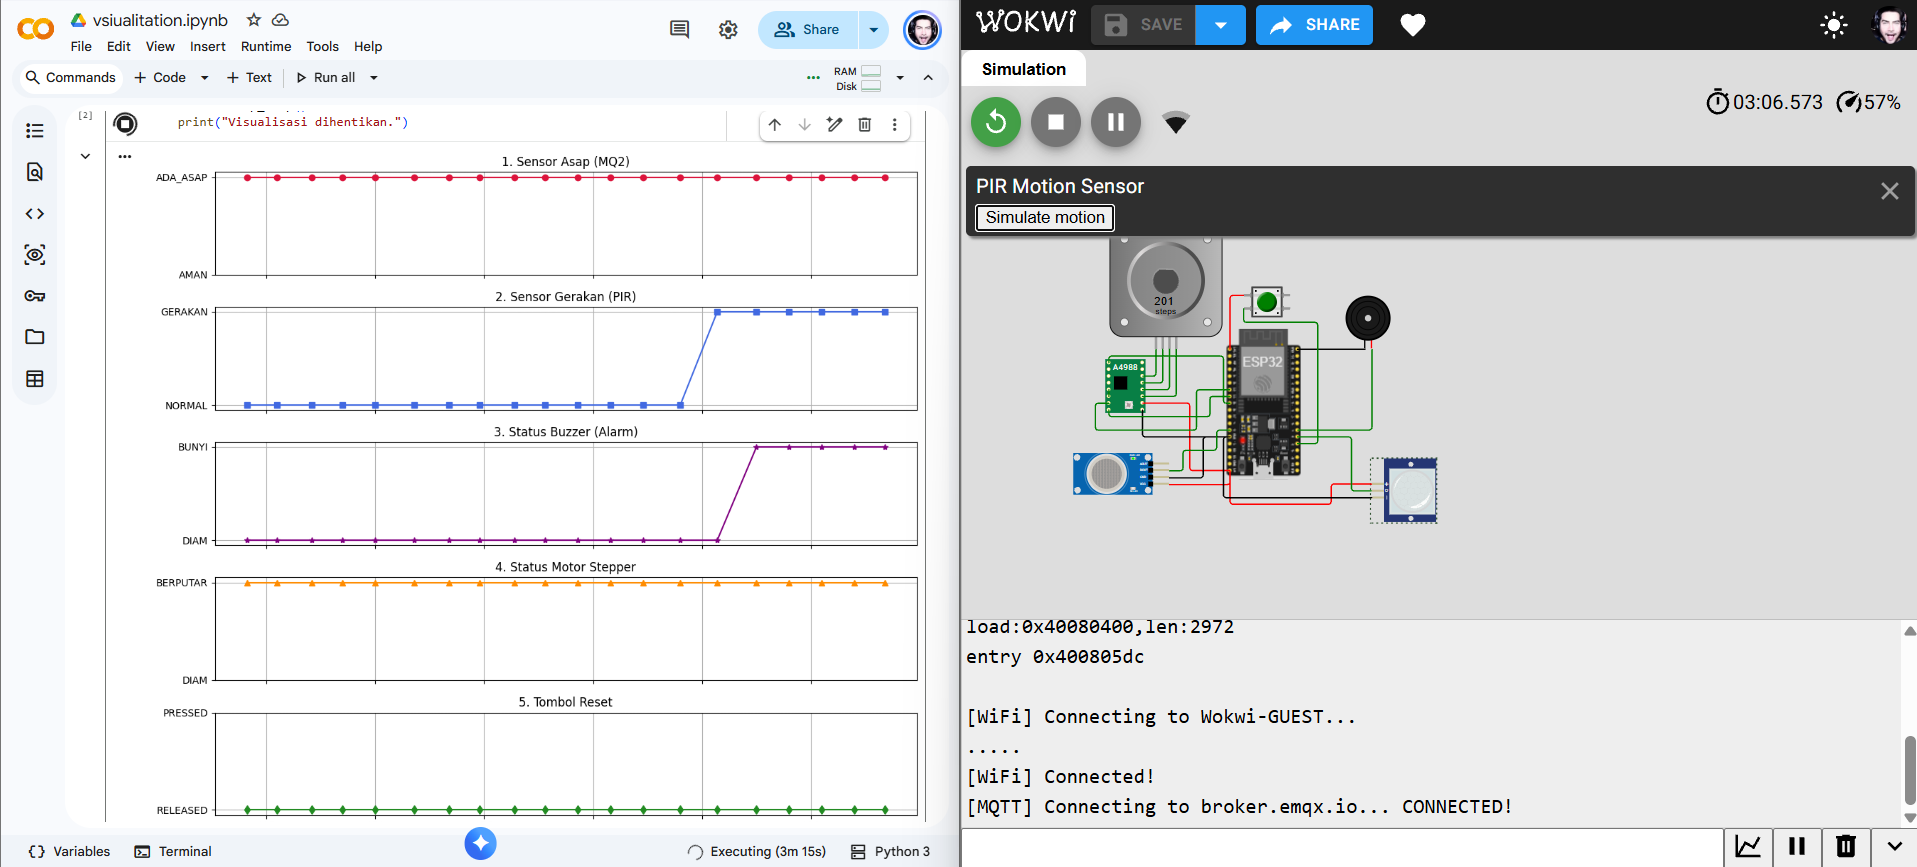
\includegraphics[width=\textwidth]{tc3.png}
  \caption{TC3: gas terdeteksi dan PIR mendeteksi gerakan}
  \label{fig:tc3}
\end{figure}

\begin{figure}[H]
  \centering
  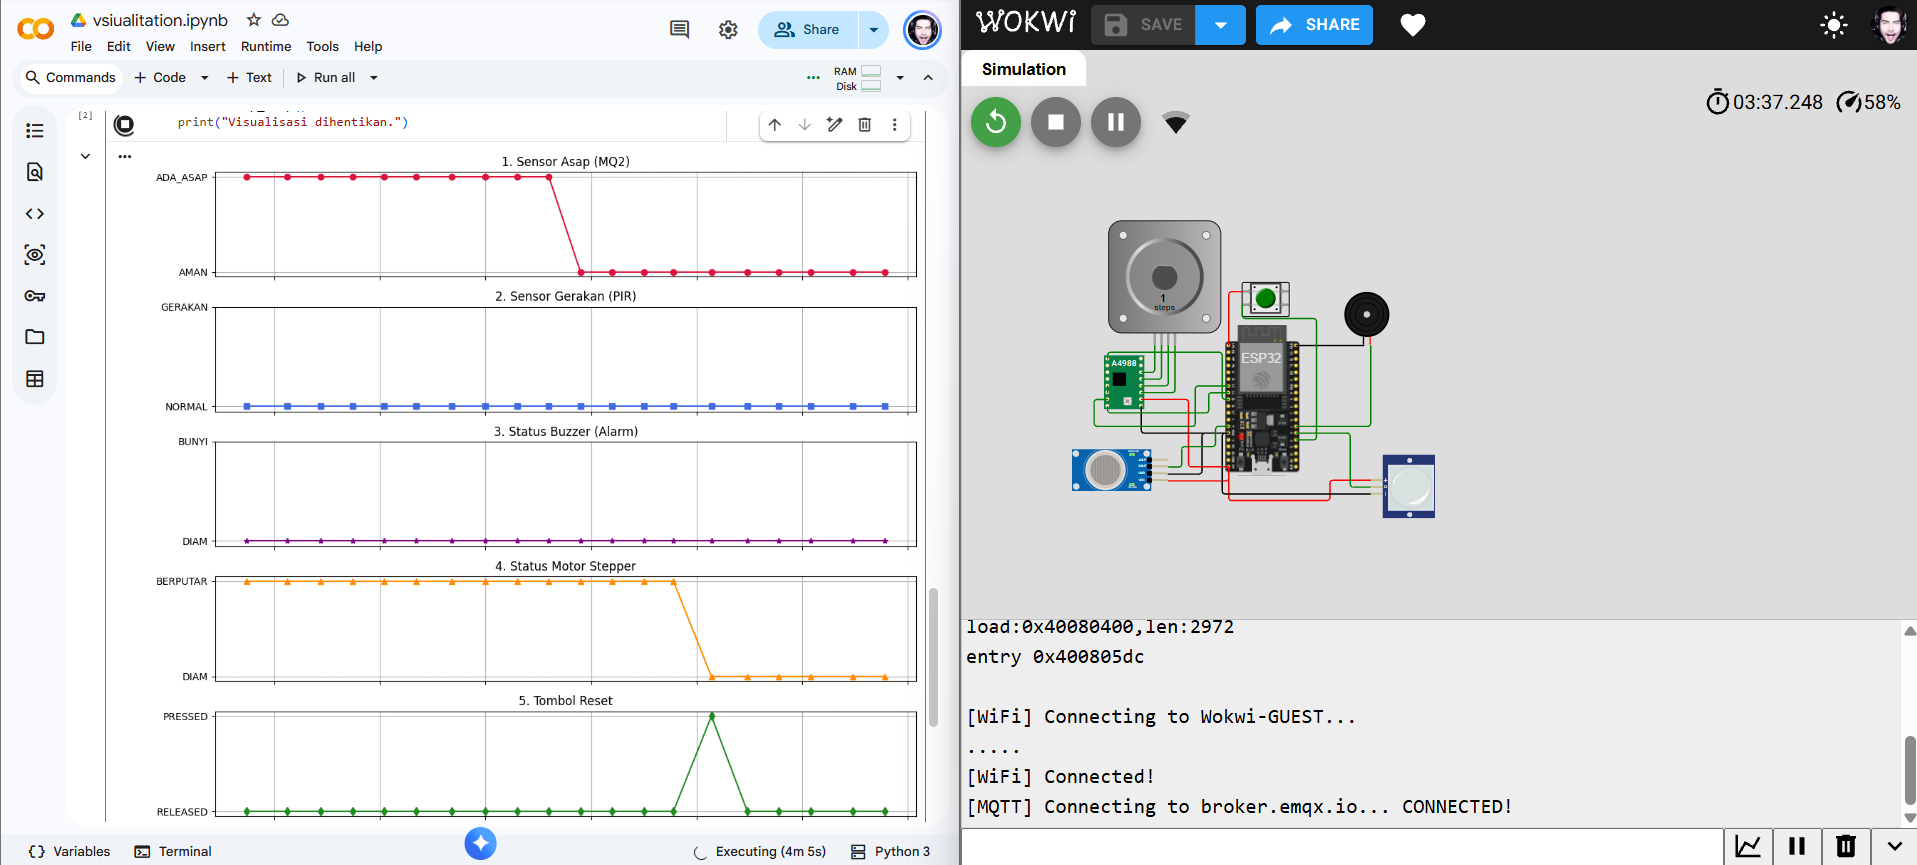
\includegraphics[width=\textwidth]{tc4.png}
  \caption{TC4: tombol reset ditekan dan sistem kembali siaga}
  \label{fig:tc4}
\end{figure}

% =========================================================================
% BAB V
% =========================================================================
\chapter{PEMBAGIAN PERAN ANGGOTA}
Proyek dikerjakan oleh empat anggota. Setiap anggota memegang satu bagian utama dari alur IoT, yaitu perancangan rangkaian dan pemrograman, simulasi dan pengujian, komunikasi dan dokumentasi, serta visualisasi data. Dengan pembagian ini, setiap tahap dalam alur sistem memiliki penanggung jawab yang jelas. Rincian peran dan kontribusi setiap anggota tercantum pada Tabel~\ref{tab:peran}.

\begin{table}[H]
  \caption{Pembagian peran anggota}
  \label{tab:peran}
  \begin{tabularx}{\textwidth}{P{2.8cm} P{2.8cm} L}
    \toprule
    \textbf{Nama Anggota} & \textbf{Peran} & \textbf{Kontribusi} \\
    \midrule
    Frenaldy Bestabba Hasugian & Dokumentasi dan Komunikasi MQTT & Menyusun laporan proyek (Bab I sampai VI, block diagram, dan lampiran). Mengatur MQTTX Web untuk memantau seluruh topic status pada broker EMQX, sekaligus memastikan pesan dari ESP32 benar-benar terkirim. \\
    \midrule
    Muhammad Sayyid Tsabit & Simulasi Wokwi dan Pengujian & Menyiapkan dan menjalankan proyek simulasi di Wokwi. Menjalankan skenario pengujian TC1 sampai TC4, lalu mendokumentasikan hasilnya dalam bentuk screenshot (Gambar~\ref{fig:tc1} sampai \ref{fig:tc4}). \\
    \midrule
    Nicholas & Perancangan Rangkaian dan Pemrograman ESP32 & Merancang rangkaian pada \texttt{diagram.json}, yang terdiri dari ESP32, sensor gas, PIR, driver A4988, motor stepper, buzzer, dan tombol reset. Menulis program \texttt{sketch.ino}, termasuk logika alarm terkunci, kendali motor stepper, dan pengiriman status melalui MQTT. \\
    \midrule
    Mitra Partogi & Dashboard dan Visualisasi Data & Membuat dashboard Google Colab dengan paho-mqtt dan Matplotlib, serta dashboard HTML. Keduanya menampilkan status gas, PIR, buzzer, motor, dan tombol secara real-time (Gambar~\ref{fig:dashboard}). \\
    \bottomrule
  \end{tabularx}
\end{table}

% =========================================================================
% BAB VI
% =========================================================================
\chapter{PENUTUP}

\section{Kesimpulan}
Sistem deteksi kebocoran gas LPG berbasis ESP32 dirancang dengan alur IoT lengkap, mulai dari \emph{sensing} dengan sensor gas MQ-2 dan PIR, logika alarm terkunci pada ESP32, aktuasi berupa motor stepper yang memutar tuas regulator ke posisi OFF dan buzzer peringatan, komunikasi melalui Serial dan MQTT ke broker publik EMQX, hingga visualisasi pada dashboard Python. Alarm terkunci memastikan sistem tidak kembali normal sebelum lokasi diperiksa. Pendekatan ini mengikuti prinsip K3: aliran gas ditutup dari sumbernya tanpa mencabut selang dan tanpa membongkar regulator.

Keempat skenario pengujian (TC1 sampai TC4) berhasil. Sistem tetap siaga saat udara normal, menutup tuas regulator saat gas terdeteksi, membunyikan buzzer hanya ketika ada orang di lokasi, dan kembali siaga setelah tombol reset ditekan. Seluruh perubahan status juga tampil pada dashboard melalui MQTT secara real-time.

\section{Pengembangan Lanjutan}
\begin{itemize}
  \item Membuat dudukan dan gir penghubung stepper ke tuas regulator pada prototipe fisik, lalu menyesuaikan jumlah langkah motor dengan sudut putar tuas dan torsi yang dibutuhkan.
  \item Mengirim notifikasi ke ponsel, misalnya melalui Telegram, ketika alarm aktif.
  \item Membaca output analog sensor MQ-2 dan mengkalibrasinya ke satuan ppm, sehingga dashboard dapat menampilkan tren kadar gas dan peringatan dini sebelum ambang tercapai.
  \item Memindahkan sensor dari strapping pin ESP32 (GPIO 0 dan 12) dan menambahkan level shifter sebelum diterapkan pada perangkat keras nyata.
  \item Mengubah program menjadi non-blocking dan membuat alarm tetap bekerja tanpa koneksi WiFi atau broker, serta memakai broker pribadi dengan autentikasi dan TLS untuk koneksi ESP32 pada produk nyata.
\end{itemize}

% =========================================================================
% LAMPIRAN
% =========================================================================
\chapter*{Lampiran}
\addcontentsline{toc}{chapter}{LAMPIRAN}

\section*{A. Tautan Proyek}
\begin{itemize}
  \item Link project Wokwi:\newline \url{https://wokwi.com/projects/479232165870904321}
  \item Source code:\newline \url{https://github.com/FrenaldyH/samsung-iot-project}
  \item Video demo:\newline \url{https://youtu.be/zDZDpb93hAY}
\end{itemize}

\section*{B. Kode Program ESP32 (sketch.ino)}
\lstinputlisting{../wokwi/sketch.ino}

\end{document}
